\documentclass[11pt,a4paper]{report}
\usepackage[textwidth=37em,vmargin=30mm]{geometry}
\usepackage{calc,xunicode,amsmath,amssymb,paralist,enumitem,tabu,booktabs,datetime2,xeCJK,xeCJKfntef,listings}
\usepackage{tocloft,fancyhdr,tcolorbox,xcolor,graphicx,eso-pic,xltxtra,xelatexemoji}

\newcommand{\envyear}[0]{2025}
\newcommand{\envdatestr}[0]{2025-05-30}
\newcommand{\envfinaldir}[0]{webdb/2025/20250530/final}

\usepackage[hidelinks]{hyperref}
\hypersetup{
    colorlinks=false,
    pdfpagemode=FullScreen,
    pdftitle={Web Digest - \envdatestr}
}

\setlength{\cftbeforechapskip}{10pt}
\renewcommand{\cftchapfont}{\rmfamily\bfseries\large\raggedright}
\setlength{\cftbeforesecskip}{2pt}
\renewcommand{\cftsecfont}{\sffamily\small\raggedright}

\setdefaultleftmargin{2em}{2em}{1em}{1em}{1em}{1em}

\usepackage{xeCJK,xeCJKfntef}
\xeCJKsetup{PunctStyle=plain,RubberPunctSkip=false,CJKglue=\strut\hskip 0pt plus 0.1em minus 0.05em,CJKecglue=\strut\hskip 0.22em plus 0.2em}
\XeTeXlinebreaklocale "zh"
\XeTeXlinebreakskip = 0pt


\setmainfont{Brygada 1918}
\setromanfont{Brygada 1918}
\setsansfont{IBM Plex Sans}
\setmonofont{JetBrains Mono NL}
\setCJKmainfont{Noto Serif CJK SC}
\setCJKromanfont{Noto Serif CJK SC}
\setCJKsansfont{Noto Sans CJK SC}
\setCJKmonofont{Noto Sans CJK SC}

\setlength{\parindent}{0pt}
\setlength{\parskip}{8pt}
\linespread{1.15}

\lstset{
	basicstyle=\ttfamily\footnotesize,
	numbersep=5pt,
	backgroundcolor=\color{black!5},
	showspaces=false,
	showstringspaces=false,
	showtabs=false,
	tabsize=2,
	captionpos=b,
	breaklines=true,
	breakatwhitespace=true,
	breakautoindent=true,
	linewidth=\textwidth
}






\newcommand{\coverpic}[2]{
    % argv: itemurl, authorname
    Cover photo by #2~~(\href{#1}{#1})
}
\newcommand{\makeheader}[0]{
    \begin{titlepage}
        % \newgeometry{hmargin=15mm,tmargin=21mm,bmargin=12mm}
        \begin{center}
            
            \rmfamily\scshape
            \fontspec{BaskervilleF}
            \fontspec{Old Standard}
            \fontsize{59pt}{70pt}\selectfont
            WEB\hfill DIGEST
            
            \vfill
            % \vskip 30pt
            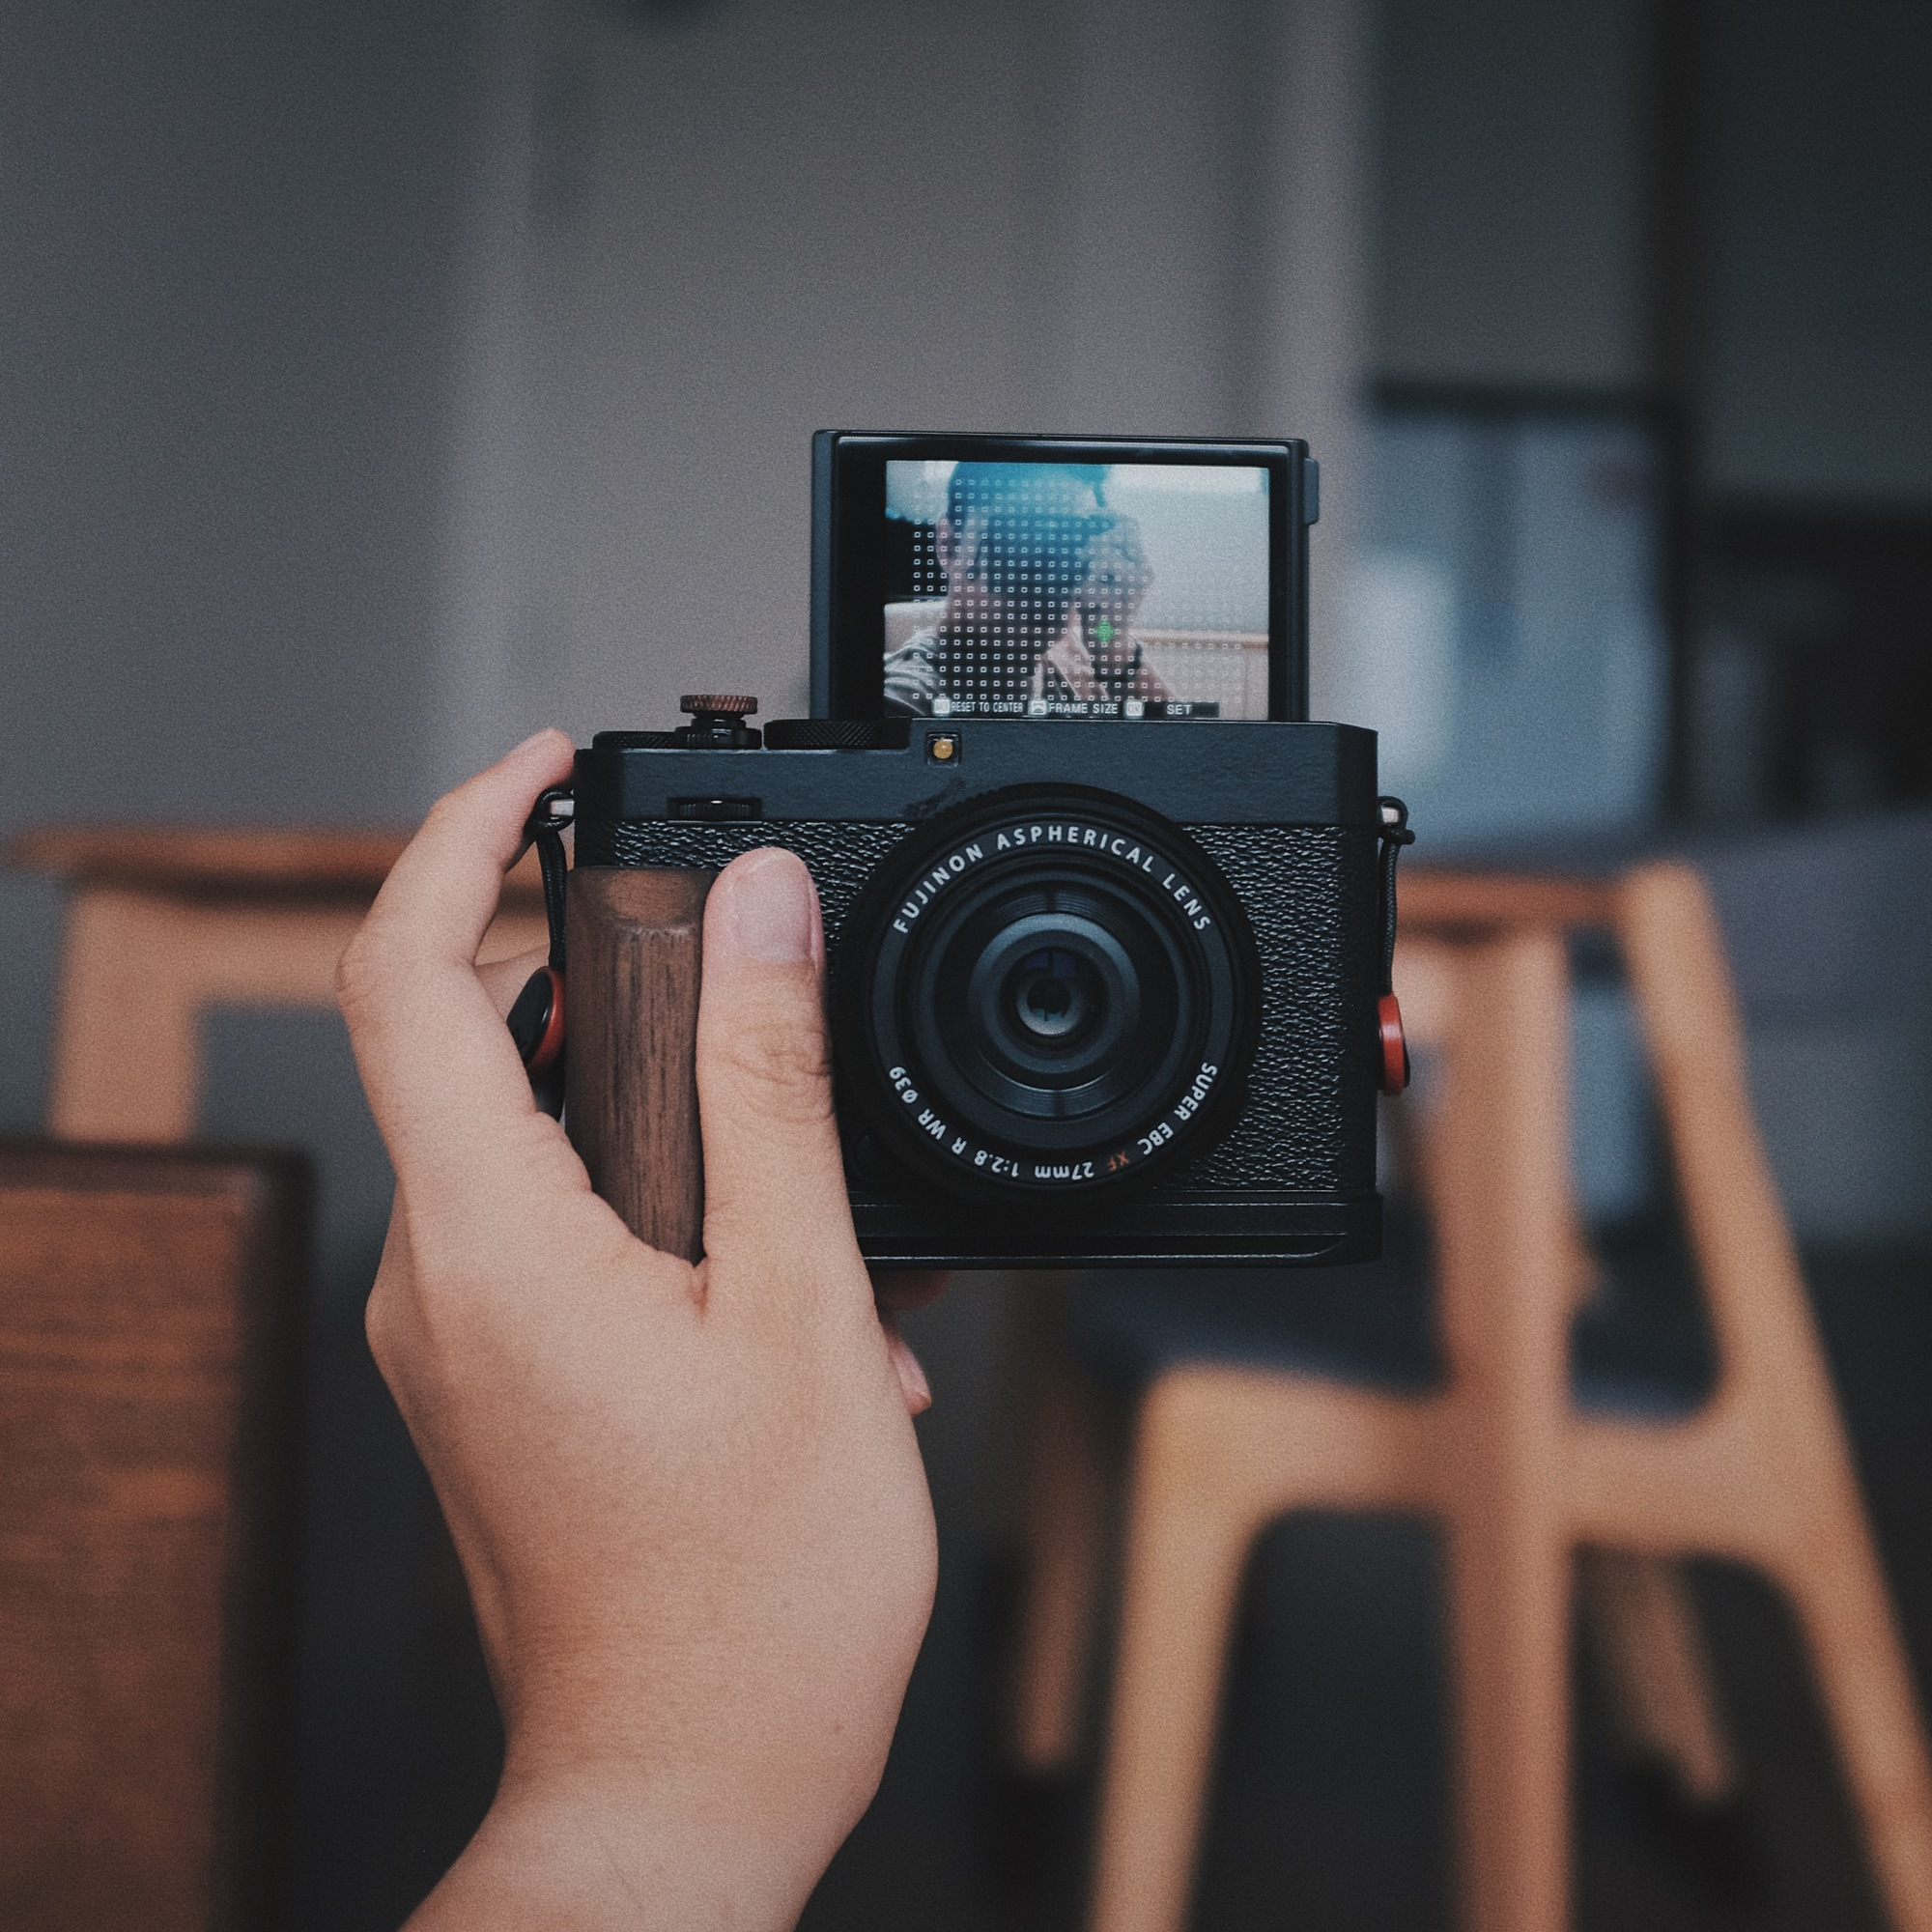
\includegraphics[width=\linewidth]{\envfinaldir/coverpic-prod.jpg}\par
            % \vskip 30pt
            \vfill

            \normalsize\rmfamily\scshape
            \copyright{} The Web Digest Project \hfill\large \envdatestr
        \end{center}
    \end{titlepage}
    % \restoregeometry
}
\newcommand{\simplehref}[1]{%
    \textcolor{blue!80!green}{\href{#1}{#1}}%
}
\renewcommand{\contentsname}{\center\Huge\sffamily\bfseries Contents\par\vskip 20pt}
\newcounter{ipartcounter}
\setcounter{ipartcounter}{0}
\newcommand{\ipart}[1]{
    % \vskip 20pt
    \clearpage
    \stepcounter{ipartcounter}
    \phantomsection
    \addcontentsline{toc}{chapter}{#1}
    % \begin{center}
    %     \Huge
    %     \sffamily\bfseries
    %     #1
    % \end{center}
    % \vskip 20pt plus 7pt
}
\newcounter{ichaptercounter}
\setcounter{ichaptercounter}{0}
\newcommand{\ichapter}[1]{
    % \vskip 20pt
    \clearpage
    \stepcounter{ichaptercounter}
    \phantomsection
    \addcontentsline{toc}{section}{\numberline{\arabic{ichaptercounter}}#1}
    \begin{center}
        \Huge
        \sffamily\bfseries
        #1
    \end{center}
    \vskip 20pt plus 7pt
}
\newcommand{\entrytitlefont}[1]{\subsection*{\raggedright\Large\sffamily\bfseries#1}}
\newcommand{\entryitemGeneric}[2]{
    % argv: title, url
    \parbox{\linewidth}{
        \entrytitlefont{#1}\par\vskip 5pt
        \footnotesize\ttfamily\mdseries
        \simplehref{#2}
    }\vskip 11pt plus 11pt minus 1pt
}
\newcommand{\entryitemGithub}[3]{
    % argv: title, url, desc
    \parbox{\linewidth}{
        \entrytitlefont{#1}\par\vskip 5pt
        \footnotesize\ttfamily\mdseries
        \simplehref{#2}\par\vskip 5pt
        \small\rmfamily\mdseries#3
    }\vskip 11pt plus 11pt minus 1pt
}
\newcommand{\entryitemAp}[3]{
    % argv: title, url, desc
    \parbox{\linewidth}{
        \entrytitlefont{#1}\par\vskip 5pt
        \footnotesize\ttfamily\mdseries
        \simplehref{#2}\par\vskip 5pt
        \small\rmfamily\mdseries#3
    }\vskip 11pt plus 11pt minus 1pt
}
\newcommand{\entryitemHackernews}[3]{
    % argv: title, hnurl, rawurl
    % \parbox{\linewidth}{
    %     \entrytitlefont{#1}\par\vskip 5pt
    %     \footnotesize\ttfamily\mdseries
    %     \simplehref{#3}\par
    %     \textcolor{black!50}{\href{#2}{#2}}
    % }\vskip 11pt plus 11pt minus 1pt
    \begin{minipage}{\linewidth}
            \entrytitlefont{#1}\par\vskip 5pt
            \footnotesize\ttfamily\mdseries
            \simplehref{#3}\par
            \textcolor{black!50}{\href{#2}{#2}}
    \end{minipage}\par\vskip 11pt plus 11pt minus 1pt
}







\begin{document}

\makeheader

\tableofcontents\clearpage




\ipart{Developers}
\ichapter{Hacker News}
\entryitemTwoLinks{Airlines are charging solo passengers higher fares than groups}{https://news.ycombinator.com/item?id=44128901}{https://thriftytraveler.com/news/airlines/airlines-charging-solo-travelers-higher-fares/}

\entryitemTwoLinks{FLUX.1 Kontext}{https://news.ycombinator.com/item?id=44128322}{https://bfl.ai/models/flux-kontext}

\entryitemTwoLinks{Human coders are still better than LLMs}{https://news.ycombinator.com/item?id=44127739}{https://antirez.com/news/153}

\entryitemTwoLinks{WeatherStar 4000+: Weather Channel Simulator}{https://news.ycombinator.com/item?id=44127109}{https://weatherstar.netbymatt.com/}

\entryitemTwoLinks{ClickHouse raises \$350M Series C}{https://news.ycombinator.com/item?id=44126753}{https://clickhouse.com/blog/clickhouse-raises-350-million-series-c-to-power-analytics-for-ai-era}

\entryitemTwoLinks{Show HN: I wrote a modern Command Line Handbook}{https://news.ycombinator.com/item?id=44126612}{https://commandline.stribny.name/}

\entryitemTwoLinks{Nova: A JavaScript and WebAssembly engine written in Rust}{https://news.ycombinator.com/item?id=44126264}{https://trynova.dev/}

\entryitemTwoLinks{Learning C3}{https://news.ycombinator.com/item?id=44125966}{https://alloc.dev/2025/05/29/learning\_c3}

\entryitemTwoLinks{Google is using AI to censor independent websites like mine}{https://news.ycombinator.com/item?id=44124820}{https://travellemming.com/perspectives/ftc-letter-google-censors-indie-publishers-with-ai/}

\entryitemTwoLinks{Show HN: I made a Zero-config tool to visualize your code}{https://news.ycombinator.com/item?id=44124652}{https://staying.fun/en}

\entryitemTwoLinks{US cancels funding for Moderna bird flu vaccine}{https://news.ycombinator.com/item?id=44124580}{https://www.reuters.com/business/healthcare-pharmaceuticals/us-cancels-more-700-million-funding-moderna-bird-flu-vaccine-2025-05-28/}

\entryitemTwoLinks{Edamagit: Magit for VSCode}{https://news.ycombinator.com/item?id=44123953}{https://github.com/kahole/edamagit}

\entryitemTwoLinks{Gurus of 90s Web Design: Zeldman, Siegel, Nielsen}{https://news.ycombinator.com/item?id=44123852}{https://cybercultural.com/p/web-design-1997/}

\entryitemTwoLinks{RSyncUI – A SwiftUI based macOS GUI for rsync}{https://news.ycombinator.com/item?id=44123289}{https://github.com/rsyncOSX/RsyncUI}

\entryitemTwoLinks{Show HN: Typed-FFmpeg 3.0–Typed Interface to FFmpeg and Visual Filter Editor}{https://news.ycombinator.com/item?id=44123098}{https://github.com/livingbio/typed-ffmpeg}

\entryitemTwoLinks{Run a C\# file directly using dotnet run app.cs}{https://news.ycombinator.com/item?id=44122582}{https://devblogs.microsoft.com/dotnet/announcing-dotnet-run-app/}

\entryitemTwoLinks{US Trade Court finds Trump tariffs illegal}{https://news.ycombinator.com/item?id=44121732}{https://www.bloomberg.com/news/articles/2025-05-28/trump-s-global-tariffs-blocked-by-us-trade-court}

\entryitemTwoLinks{HTAP is Dead}{https://news.ycombinator.com/item?id=44121177}{https://www.mooncake.dev/blog/htap-is-dead}

\entryitemTwoLinks{Long live American Science and Surplus}{https://news.ycombinator.com/item?id=44120507}{https://milwaukeerecord.com/city-life/long-live-american-science-surplus-which-needs-your-help/}

\entryitemTwoLinks{A visual exploration of vector embeddings}{https://news.ycombinator.com/item?id=44120306}{http://blog.pamelafox.org/2025/05/a-visual-exploration-of-vector.html}\ichapter{Phoronix}
\entryitemGeneric{\hskip 0pt{}Linux 6.16 Adds Support For Graceful Host Removal For eMMC \& SD Cards}{https://www.phoronix.com/news/Linux-6.16-eMMC-SD-Graceful}

\entryitemGeneric{\hskip 0pt{}NVIDIA 575.57.08 Linux Stable Driver Released With Smooth Motion \& Other Updates}{https://www.phoronix.com/news/NVIDIA-575.57.08-Linux}

\entryitemGeneric{\hskip 0pt{}Linux 6.16 Networking Brings Some Big Performance Improvements \& OpenVPN Driver}{https://www.phoronix.com/news/Linux-6.16-Networking}

\entryitemGeneric{\hskip 0pt{}AMD EPYC 4585PX \& EPYC 4565P With DDR5-4800 vs. DDR5-5600 Performance}{https://www.phoronix.com/review/amd-epyc-4005-ddr5-benchmarks}

\entryitemGeneric{\hskip 0pt{}KDE Plasma 6.4 Beta 2 Brings XWayland Fixes}{https://www.phoronix.com/news/KDE-Plasma-6.4-Beta-2}

\entryitemGeneric{\hskip 0pt{}Linux 6.16 Crypto Brings Faster AES-XTS On AVX-512 CPUs, Intel QAT Gen6 Support}{https://www.phoronix.com/news/Linux-6.16-Crypto}

\entryitemGeneric{\hskip 0pt{}Out-Of-Date OpenH264 On Fedora Is Frustrating Users With A High Severity CVE}{https://www.phoronix.com/news/Fedora-OpenH264-Security-Woe}

\entryitemGeneric{\hskip 0pt{}EROFS Lands Support For Tapping Intel QAT Accelerators}{https://www.phoronix.com/news/Linux-6.16-EROFS-Intel-QAT}

\entryitemGeneric{\hskip 0pt{}Canonical To Release Monthly Ubuntu Snapshots For Testing \& Building Out Automation}{https://www.phoronix.com/news/Monthly-Ubuntu-Snapshots}\ichapter{Dribbble}
\entryitemGeneric{\hskip 0pt{}Create email inbox composition}{https://dribbble.com/shots/26083118-Create-email-inbox-composition}

\entryitemGeneric{\hskip 0pt{}Eagle}{https://dribbble.com/shots/26085536-Eagle}

\entryitemGeneric{\hskip 0pt{}Patriot Logo Design (Unused for Sale)}{https://dribbble.com/shots/26081047-Patriot-Logo-Design-Unused-for-Sale}

\entryitemGeneric{\hskip 0pt{}Heliopoint}{https://dribbble.com/shots/26081987-Heliopoint}

\entryitemGeneric{\hskip 0pt{}Apple}{https://dribbble.com/shots/26084067-Apple}

\entryitemGeneric{\hskip 0pt{}B2B Dashboard \& Web App UI UX Design for Carbon Solutions}{https://dribbble.com/shots/26076624-B2B-Dashboard-Web-App-UI-UX-Design-for-Carbon-Solutions}

\entryitemGeneric{\hskip 0pt{}Heyo Turns 2!}{https://dribbble.com/shots/26078572-Heyo-Turns-2}

\entryitemGeneric{\hskip 0pt{}Roaring Bear}{https://dribbble.com/shots/26077332-Roaring-Bear}

\entryitemGeneric{\hskip 0pt{}Smart Home App}{https://dribbble.com/shots/26076565-Smart-Home-App}

\entryitemGeneric{\hskip 0pt{}Fox Brand Mascot}{https://dribbble.com/shots/26077954-Fox-Brand-Mascot}

\entryitemGeneric{\hskip 0pt{}Europe Logo Concept}{https://dribbble.com/shots/26077297-Europe-Logo-Concept}

\entryitemGeneric{\hskip 0pt{}Mobile App Design – Language Learning}{https://dribbble.com/shots/26076418-Mobile-App-Design-Language-Learning}

\entryitemGeneric{\hskip 0pt{}HYDRO - Logo Design}{https://dribbble.com/shots/26073470-HYDRO-Logo-Design}

\entryitemGeneric{\hskip 0pt{}Credit payment card bank app animation}{https://dribbble.com/shots/26063214-Credit-payment-card-bank-app-animation}

\entryitemGeneric{\hskip 0pt{}Kloak Wordmark}{https://dribbble.com/shots/26073220-Kloak-Wordmark}

\entryitemGeneric{\hskip 0pt{}Project Management Dashboard}{https://dribbble.com/shots/26070177-Project-Management-Dashboard}

\entryitemGeneric{\hskip 0pt{}Perception web design}{https://dribbble.com/shots/25995935-Perception-web-design}

\entryitemGeneric{\hskip 0pt{}Stanley // Website}{https://dribbble.com/shots/26056691-Stanley-Website}

\entryitemGeneric{\hskip 0pt{}i SEA you}{https://dribbble.com/shots/26062936-i-SEA-you}

\entryitemGeneric{\hskip 0pt{}AltSocial}{https://dribbble.com/shots/26060858-AltSocial}

\entryitemGeneric{\hskip 0pt{}Fariland Headwear Symbol}{https://dribbble.com/shots/26063219-Fariland-Headwear-Symbol}

\entryitemGeneric{\hskip 0pt{}Glassmorphic 3D Logo Animation}{https://dribbble.com/shots/26061835-Glassmorphic-3D-Logo-Animation}

\entryitemGeneric{\hskip 0pt{}Animals illustration}{https://dribbble.com/shots/26037153-Animals-illustration}

\entryitemGeneric{\hskip 0pt{}Mobile App UI — HR \& Hiring Platform Design}{https://dribbble.com/shots/26061833-Mobile-App-UI-HR-Hiring-Platform-Design}


\ipart{Developers~~~~(zh-Hans)}
\ichapter{Solidot}
\entryitemGeneric{\hskip 0pt{}美国将撤销中国留学生签证}{https://www.solidot.org/story?sid=81420}

\entryitemGeneric{\hskip 0pt{}xAI 支付 3 亿美元让 Telegram 集成 Grok}{https://www.solidot.org/story?sid=81419}

\entryitemGeneric{\hskip 0pt{}我们如何失去互联网?}{https://www.solidot.org/story?sid=81418}

\entryitemGeneric{\hskip 0pt{}海洋在变暗}{https://www.solidot.org/story?sid=81417}

\entryitemGeneric{\hskip 0pt{}几乎所有成年美国人盐摄入量都超过建议量}{https://www.solidot.org/story?sid=81416}

\entryitemGeneric{\hskip 0pt{}苹果收购了第一家游戏工作室 RAC7 }{https://www.solidot.org/story?sid=81415}

\entryitemGeneric{\hskip 0pt{}牙本质起源于古鱼外骨骼中的感觉组织}{https://www.solidot.org/story?sid=81414}

\entryitemGeneric{\hskip 0pt{}重大科学突破越来越难以实现}{https://www.solidot.org/story?sid=81413}

\entryitemGeneric{\hskip 0pt{}免疫反应在白天更强}{https://www.solidot.org/story?sid=81412}

\entryitemGeneric{\hskip 0pt{}特朗普政府考虑对留学生进行社交媒体审查}{https://www.solidot.org/story?sid=81411}

\entryitemGeneric{\hskip 0pt{}逾 2\% 美国人服用 GLP-1 减肥药}{https://www.solidot.org/story?sid=81410}

\entryitemGeneric{\hskip 0pt{}银河系的一根``骨骼''被脉冲星撞断}{https://www.solidot.org/story?sid=81409}

\entryitemGeneric{\hskip 0pt{}The Browser Company 停止开发 Arc 转向 AI 驱动浏览器 Dia }{https://www.solidot.org/story?sid=81408}

\entryitemGeneric{\hskip 0pt{}AI 模型出现崩溃迹象}{https://www.solidot.org/story?sid=81407}

\entryitemGeneric{\hskip 0pt{}BGP 系统的 Bug 处理方式导致部分网络故障}{https://www.solidot.org/story?sid=81406}

\entryitemGeneric{\hskip 0pt{}鹰利用交通灯捕猎}{https://www.solidot.org/story?sid=81405}

\entryitemGeneric{\hskip 0pt{}腾讯将成为 K-Pop 经纪公司 SM娱乐的第二大股东}{https://www.solidot.org/story?sid=81404}

\entryitemGeneric{\hskip 0pt{}台积电下注基于 MicroLED 的光互联技术}{https://www.solidot.org/story?sid=81403}

\entryitemGeneric{\hskip 0pt{}金星共轨小行星可能威胁到地球}{https://www.solidot.org/story?sid=81402}

\entryitemGeneric{\hskip 0pt{}CIA 曾经秘密运营了一家星球大战粉丝网站}{https://www.solidot.org/story?sid=81401}\ichapter{V2EX}
\entryitemGeneric{\hskip 0pt{}[阅读] 书荒,求书籍推荐}{https://www.v2ex.com/t/1135309}

\entryitemGeneric{\hskip 0pt{}[创业组队] 寻后端架构与开发( PHP 和 GO)}{https://www.v2ex.com/t/1135308}

\entryitemGeneric{\hskip 0pt{}[酷工作] 招远程全职后端主程( PHP /GOlang), 4000 美金/月+分红}{https://www.v2ex.com/t/1135307}

\entryitemGeneric{\hskip 0pt{}[Apple] mac 下使用 vscode 远程内网的 Linux 进行远程开发 效果如何?}{https://www.v2ex.com/t/1135306}

\entryitemGeneric{\hskip 0pt{}[问与答] 求助:Claude3.7/4.0 执行复杂任务时如何保证代码的连续性}{https://www.v2ex.com/t/1135305}

\entryitemGeneric{\hskip 0pt{}[问与答] 我想老实人维权,找了正规法院,二审终审还是判输,你该怎么办?}{https://www.v2ex.com/t/1135304}

\entryitemGeneric{\hskip 0pt{}[酷工作] [携程 Trip.com] 内推|后端开发专家|旅游 BU|上海| Java 方向|高质量团队氛围}{https://www.v2ex.com/t/1135303}

\entryitemGeneric{\hskip 0pt{}[程序员] 20 种数组去重的方法}{https://www.v2ex.com/t/1135302}

\entryitemGeneric{\hskip 0pt{}[分享发现] 关于网络统一认证,大家还记得十一年前的手机卡强制实名吗}{https://www.v2ex.com/t/1135301}

\entryitemGeneric{\hskip 0pt{}[硬件] 有没有能将视角内的英文自动翻译成中文的智能眼镜}{https://www.v2ex.com/t/1135300}

\entryitemGeneric{\hskip 0pt{}[iPhone] 你们的 iPhone 有自动重启桌面吗?}{https://www.v2ex.com/t/1135297}

\entryitemGeneric{\hskip 0pt{}[Apple] 果子是在抽什么风, wifi 支持规格居然不是线性迭代的}{https://www.v2ex.com/t/1135293}

\entryitemGeneric{\hskip 0pt{}[分享创造] 面向 vibe coding 的 product hunt}{https://www.v2ex.com/t/1135292}

\entryitemGeneric{\hskip 0pt{}[职场话题] 吐槽下公司,不知道是我有问题,还是公司有问题}{https://www.v2ex.com/t/1135291}

\entryitemGeneric{\hskip 0pt{}[问与答] 不懂就问,有些网站在开发者工具看没有 api 的调用,网站的数据是哪里来的?}{https://www.v2ex.com/t/1135289}

\entryitemGeneric{\hskip 0pt{}[问与答] yahoo 如何注册?}{https://www.v2ex.com/t/1135288}

\entryitemGeneric{\hskip 0pt{}[问与答] 浙江省个体户有没有人搞定了核定征收方式的税务申报}{https://www.v2ex.com/t/1135287}

\entryitemGeneric{\hskip 0pt{}[Apple] appletv 显示的带宽为什么超过了实际带宽?}{https://www.v2ex.com/t/1135286}

\entryitemGeneric{\hskip 0pt{}[职场话题] 你们做远程职位怎么保证安全的?多长时间发一次工资?如果按月发工资,怎么防止干一个月对方跑路了要不到钱?}{https://www.v2ex.com/t/1135284}

\entryitemGeneric{\hskip 0pt{}[酷工作] [广州] [内推] 分布式数据库与算法模型落地经验的后端研发}{https://www.v2ex.com/t/1135283}

\entryitemGeneric{\hskip 0pt{}[问与答] 限额背景下关于日常用卡}{https://www.v2ex.com/t/1135282}

\entryitemGeneric{\hskip 0pt{}[VPS] 有没有要合租搬瓦工的 vps}{https://www.v2ex.com/t/1135281}

\entryitemGeneric{\hskip 0pt{}[问与答] 苦于对家具/电器的认识不够,请教大家建议?}{https://www.v2ex.com/t/1135280}

\entryitemGeneric{\hskip 0pt{}[路由器] 求推荐个路由器. 只做 AP}{https://www.v2ex.com/t/1135279}

\entryitemGeneric{\hskip 0pt{}[Apple] 外区 Apple ID 可以用来做主账号吗?}{https://www.v2ex.com/t/1135277}

\entryitemGeneric{\hskip 0pt{}[问与答] 抖音通过哪些 api 接口判断 ip 归属}{https://www.v2ex.com/t/1135276}

\entryitemGeneric{\hskip 0pt{}[问与答] 有什么好办法把百度网盘的内容转移到夸克网盘}{https://www.v2ex.com/t/1135275}

\entryitemGeneric{\hskip 0pt{}[分享创造] 产品经理业余用 AI 写的网站-细分垂直领域}{https://www.v2ex.com/t/1135274}

\entryitemGeneric{\hskip 0pt{}[macOS] Win 刚转 MacOS 寻求好用工具}{https://www.v2ex.com/t/1135273}

\entryitemGeneric{\hskip 0pt{}[汽车] 智界 R7 值得入手吗}{https://www.v2ex.com/t/1135272}

\entryitemGeneric{\hskip 0pt{}[问与答] StartAllBack(开始菜单增强工具) v3.9.9.5271 与 Windows 11 24H2(OS 内部版本: 26100.4202)不兼容,回退到 3.9.7 任务栏能显示}{https://www.v2ex.com/t/1135271}

\entryitemGeneric{\hskip 0pt{}[职场话题] 代面试是什么情况}{https://www.v2ex.com/t/1135270}

\entryitemGeneric{\hskip 0pt{}[全球工单系统] 高德地图驾车导航,行驶到 1km 时自动结束导航。}{https://www.v2ex.com/t/1135269}

\entryitemGeneric{\hskip 0pt{}[VXNA] 申请收录个人博客-燃雄}{https://www.v2ex.com/t/1135268}

\entryitemGeneric{\hskip 0pt{}[推广] 微信支付商家收款码 0.3\%费率免费开通}{https://www.v2ex.com/t/1135267}

\entryitemGeneric{\hskip 0pt{}[问与答] 代理开启上网问题}{https://www.v2ex.com/t/1135266}

\entryitemGeneric{\hskip 0pt{}[Visual Studio Code] 助力 vscode 开放布局调整 api}{https://www.v2ex.com/t/1135265}

\entryitemGeneric{\hskip 0pt{}[随想] 由``恶意划车''贴想到的小孩子教育问题}{https://www.v2ex.com/t/1135264}

\entryitemGeneric{\hskip 0pt{}[Windows] 终于解决了 win11 输入法在切换窗口的时候时不时随机切换输入法状态的问题🤣}{https://www.v2ex.com/t/1135262}

\entryitemGeneric{\hskip 0pt{}[宽带症候群] 移动晚高峰的白名单 QoS 限速}{https://www.v2ex.com/t/1135261}

\entryitemGeneric{\hskip 0pt{}[问与答] 老站长打算转行拍视频与做主播了,有什么好方向可以选?}{https://www.v2ex.com/t/1135260}

\entryitemGeneric{\hskip 0pt{}[分享创造] iOS 程序员还有什么出路啊,给兄弟们丢脸了}{https://www.v2ex.com/t/1135258}

\entryitemGeneric{\hskip 0pt{}[酷工作] 「招聘」「实习」苏州徕卡显微软开}{https://www.v2ex.com/t/1135256}

\entryitemGeneric{\hskip 0pt{}[问与答] 你们接到骚扰电话是如何处理的?}{https://www.v2ex.com/t/1135255}

\entryitemGeneric{\hskip 0pt{}[酷工作] [深圳][内推] shopify 前端工程师 / 海外电商高级设计}{https://www.v2ex.com/t/1135254}

\entryitemGeneric{\hskip 0pt{}[酷工作] [招聘] [前端、后端、运营、产品] [集换社] TCG 技术团队扩编 | 用代码重塑卡牌交易生态}{https://www.v2ex.com/t/1135253}

\entryitemGeneric{\hskip 0pt{}[分享发现] 想创建一个 cursor 使用分享群,用来分享交流 cursor,老规矩还是复古的 QQ 群: 374366847}{https://www.v2ex.com/t/1135252}

\entryitemGeneric{\hskip 0pt{}[投资] 炒股心态崩了}{https://www.v2ex.com/t/1135251}

\entryitemGeneric{\hskip 0pt{}[云计算] 告别阿里云:一个合作十年以上老用户的心碎经历}{https://www.v2ex.com/t/1135250}

\entryitemGeneric{\hskip 0pt{}[日本] 当前(2025)在日本用得多的类似于大众点评的 App?}{https://www.v2ex.com/t/1135249}


\ipart{Generic News}
\ichapter{AP News}
\entryitemWithDescription{\hskip 0pt{}Victoria's Secret US website is down as lingerie seller addresses `security incident'}{https://apnews.com/article/c870000e7ae21369df52a5347626435d}{}

\entryitemWithDescription{\hskip 0pt{}AP PHOTOS: Replica of ship sailed by Christopher Columbus in 1492 docks in London}{https://apnews.com/article/1464fbb05954192ffdd58bcb9e6988a5}{}

\entryitemWithDescription{\hskip 0pt{}Ford recalls more than a million vehicles for software glitch that makes rearview camera unreliable}{https://apnews.com/article/95c4b06d0ef6d7b86b96c17fb8fee9a5}{}

\entryitemWithDescription{\hskip 0pt{}Cosmetics company E.l.f acquires Hailey Bieber's Rhode beauty brand for \$1 billion}{https://apnews.com/article/e50afe56cd3d7e6caa004bcc7eeb420b}{}

\entryitemWithDescription{\hskip 0pt{}Search suspended for a missing man in Swiss glacier collapse that destroyed 90\% of an Alpine village}{https://apnews.com/article/642e4cfa0beccdcd744e146d36285027}{}

\entryitemWithDescription{\hskip 0pt{}Ancient DNA reveals a new group of people who lived near land bridge between the Americas}{https://apnews.com/article/dd65182aa1bd08621b7c348145ade272}{}

\entryitemWithDescription{\hskip 0pt{}Alpine village is largely destroyed when a Swiss glacier collapses}{https://apnews.com/article/28e15e240eacb40bcbdb6a8f15d49398}{}

\entryitemWithDescription{\hskip 0pt{}Tiger's son, Charlie Woods, wins Team TaylorMade Invitational in claiming 1st AJGA event}{https://apnews.com/article/c30f0fdeb6cf8878b3b521caab232247}{}

\entryitemWithDescription{\hskip 0pt{}Patriots say they will handle video of receiver Stefon Diggs internally}{https://apnews.com/article/93182b80cfdc518198271fe4b3fe88e8}{}

\entryitemWithDescription{\hskip 0pt{}Cats with hooked and bent tails fill Nagasaki, Japan, where they are thought to bring good luck}{https://apnews.com/article/8f81c1262cea38b35d2ff167b33adb9b}{}

\entryitemWithDescription{\hskip 0pt{}As more Argentines go childless, pampered dogs become part of the family}{https://apnews.com/article/c1fb28f904ee06d1d8752aee6116ff17}{}

\entryitemWithDescription{\hskip 0pt{}Billion dollar pizza? Bitcoin soars on key anniversary of crypto's growth}{https://apnews.com/article/9288849c8a3a9767c3b552021f32c509}{}

\entryitemWithDescription{\hskip 0pt{}George Wendt, who played beloved barfly Norm on `Cheers' and found another home onstage, dies at 76}{https://apnews.com/article/55681263ea8b5bddaf1c89e8e9ba8cb1}{}






\clearpage
\leavevmode\vfill
\footnotesize

Copyright \copyright{} 2023-2025 Neruthes and other contributors.

This document is published with CC BY-NC-ND 4.0 license.

The entries listed in this newsletter may be copyrighted by their respective creators.

This newsletter is generated by the Web Digest project.

The newsletters are also delivered via Telegram channel \CJKunderline{\href{https://t.me/webdigestchannel}{https://t.me/webdigestchannel}}.\\
RSS feed is available at \CJKunderline{\href{https://webdigest.pages.dev/rss.xml}{https://webdigest.pages.dev/rss.xml}}.

This newsletter is available in PDF at
\CJKunderline{\href{https://webdigest.pages.dev/}{https://webdigest.pages.dev/}}.

The source code being used to generate this newsletter is available at\\
\CJKunderline{\href{https://github.com/neruthes/webdigest}{https://github.com/neruthes/webdigest}}.

This newsletter is also available in
\CJKunderline{\href{http://webdigest.pages.dev/readhtml/\envyear/WebDigest-20250530.html}{HTML}} and
\CJKunderline{\href{https://github.com/neruthes/webdigest/blob/master/markdown/\envyear/WebDigest-20250530.md}{Markdown}}.


\coverpic{https://unsplash.com/photos/mountains-and-lakes-are-shrouded-in-mist-8xXFONfEUtA}{Dario Jud}


\end{document}
